\documentclass[12pt]{article}
%\renewcommand{\thesection}{}
\usepackage{mathtools}
\usepackage{commath}
\usepackage[sc,osf]{mathpazo}
\usepackage{tikz}
\usetikzlibrary{positioning}
\usepackage{wrapfig}

%\usepackage{fontspec}
%\setmainfont{Humor-Sans}

\usepackage{amsmath}
\usepackage{amsthm}
\usepackage{graphicx}
%\usepackage[plain]{algorithm}
%\usepackage{algorithmic}

\usepackage{amsfonts}
\usepackage{amssymb}
\usepackage{amsthm}
\usepackage{mathtools}

%\usepackage[noend]{algorithmic} 
\usepackage{algorithmic} 
\usepackage{algorithm,caption}
\algsetup{indent=2em} 
\renewcommand{\algorithmiccomment}[1]{\hspace{2em}// #1} 

\newtheorem*{thm}{Theorem}



\usepackage{hyperref}
\hypersetup{
	colorlinks=false,
	linkcolor=red,
	filecolor=red,      
	urlcolor=red,
}

\urlstyle{same}



\begin{document}
	
	   
	     
	
		\enlargethispage{2cm}
		
		\begin{center}
			
			\vspace*{-1cm}
			
			\textbf{\Large Notes on Machine Learning     }(work in progress)\\[10pt]
			

\textbf{\Large Aswin}\\ [8pt]			
			
			\end{center}
		
\cleardoublepage

\tableofcontents
\newpage

\section{Overview}

I made this document as a way to learn ML for my Maters' thesis . It’s not an original work, but a compilation of scribed notes of the ML course by Dr Sanjoy Dasgupta(UCSD), [SD] which I audited. Some parts are drawn directly/inspired from Andrew NG's Stanford CS229 course notes, [ANG] and Kilian weinberger's Cornell CS4780 course notes[KW]. My primary reference was 'The Elements of Statistical Learning' by Trevor Hastie, Robert Tibshirani, Jerome Friedman[HTF]. So there will be considerable overlap with the aforementioned materials. This note might lack mathematical rigor but I have tried to give proofs and supplementary topics wherever necessary. For each algorithm, I have given a url to Github repo containing the implemetation using one of the three datasets viz Fisher's Iris dataset, Wisconsin Breast Cancer Dataset and MNIST handwritten digits dataset.
Please write to me if you find any inaccuracies.I hope this   proves at least moderately
interesting or useful for you.

\cleardoublepage







\section[title]{Intro to Neural Networks \footnote{A compilation of scribed notes of 11-785 Intro to DL, CMU and Andrew NG's Coursera course along with inputs from  the book 'Deep Learning' by Goodfellow, Bengio and Courville }}


The linear models mentioned earlier have serious shortcomings as in inability to learn interaction between any  two input variables.\ To extend linear models to represent nonlinear functions of x, we can apply
the linear model not to x itself but to a transformed input $\phi(x)$, where $\phi$ is a nonlinear transformation. In the linear models, say for example logistic regression  the model learns the parameters (weights and bias) but neural network learns the representation $\phi$ in addition to the parameters.

The strategy of deep learning is to learn $\phi$. In this approach, we have a model
$y = f (x; \theta , w ) = \phi(x; \theta)^{T} w $. We now have parameters $\theta$ that we use to learn
$\phi$ from a broad class of functions, and parameters w that map from $\phi(x)$ to
the desired output. This is an example of a deep feedforward network, with
$\phi$ defining a hidden layer.We parametrize the representation as $\phi(x;\theta)$ and use the optimization algorithm to find the $\theta$ that corresponds to a good representation. In general we can write 

$$h : \phi(x) \rightarrow \phi(x)^T w + b$$ where $\phi(x)$ =  $\sigma(U\vec{x} )$, $\sigma$ is a transition function.
But we can argue that the transformation $x \rightarrow \phi(x)$ can be attained by a cascade of arbitrary number of  transformation say,\ $x \rightarrow \phi^{''}(x) \rightarrow \phi^{'}(x) \rightarrow \phi (x)$




$$\phi(x)  =  \sigma(U^{'} \phi^{'}(x))$$  
$$\phi^{'}(x)  =  \sigma(U^{''} \phi^{''}(x))$$ 
$$\phi^{''}(x) = \sigma(Ux)$$

\cleardoublepage

 \section{Perceptron Recap}

In a binary classification problem , where dataset(D) is  $(x,y) \in \mathbb{R}^{d} \times\{-1,1\}$, the  learning problem is to find a hyperplane which separates the data into two classes, 
assuming the data is linearly classifiable. The hyperplane is parametrized by $w\in\mathbb{R}^{d}$ and $ b \in \mathbb{R}$ such that $w.x + b = 0 $, so the poblem is equivalent to learning  the parameters $w$ and $b$.On point $x$, we predict the label as $\textbf{sign(w.x + b)}$.\\
$$(w.x + b) > 0  \implies y = +1 \therefore y(w.x + b) > 0 $$

$$(w.x + b) < 0  \implies y = -1 \therefore y(w.x + b) > 0 $$

i.e., If the true label of x is y, then $y(w.x + b) > 0 $, whereas for a misclassified pointi$y(w.x + b) \leq 0 $.\\







Perceptron can be loosely thought of as a threshold gate very much like a biological neuron as in when the weighted sum of the inputs (voltage analogue) exceeds the threshold $T$, the perceptron's output is identically one (neuron fires) else zero always(rest state neuron). This is shown in Fig.1.

\begin{figure}[h]
	\centering
	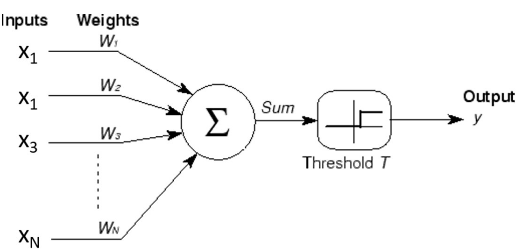
\includegraphics[width=0.5\linewidth]{img/perceptron}
	\caption{}
	\label{fig:perceptron}
\end{figure}

\cleardoublepage

The output of such a perceptron will be a step function, such that 



\begin{equation} 
y =
\begin{cases}
1, & \text{if} \  \sum_{i} w_ix_i \geq T 
\\
0 , &   else 
\end{cases}
\end{equation}


If we define $z = \sum_{i} w_ix_i - T $, then it is equivalent to,

\begin{equation} 
y =
\begin{cases}
1, & \text{if} \ z \geq 0 
\\
0 , &   else 
\end{cases}
\end{equation}


This threshold gate can realize AND and OR GATE, but not XOR gate.

\subsection{Multi-layer Perceptron}

MLP  is a network of perceptrons.Generically a MLP can be said to have three different types of layers, the input layer, output layer and the hidden layer.The input layer doesnt contain perceptrons. The nodes in the  input layer represent each components of the input data vector.The output layer gives the output. Flanked by these two are the hidden layer. The inpput and output of a  MLP can be real valued or Boolean. \\ 

\tikzset{%
	every neuron/.style={
		circle,
		draw,
		minimum size=1cm
	},
	neuron missing/.style={
		draw=none, 
		scale=4,
		text height=0.333cm,
		execute at begin node=\color{black}$\vdots$
	},
}

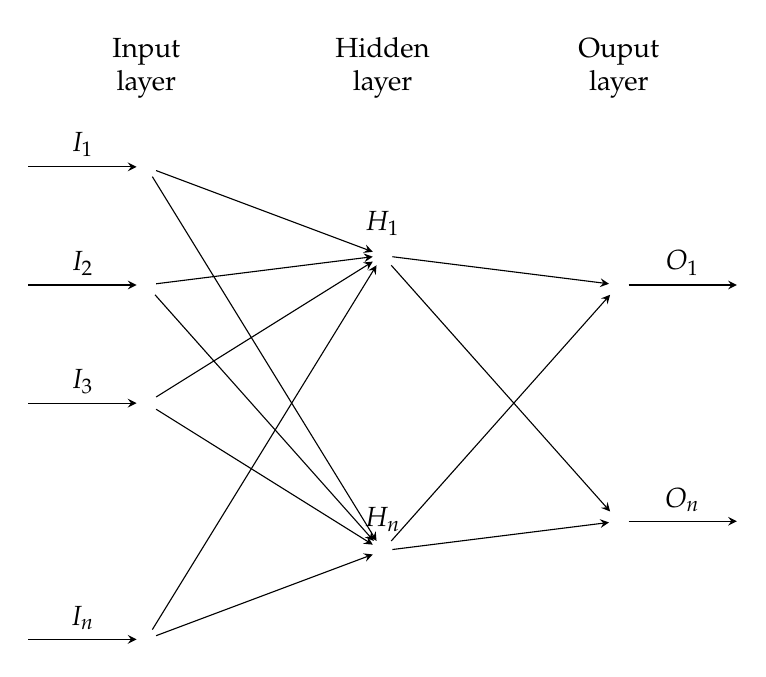
\begin{tikzpicture}[x=1.5cm, y=1.5cm, >=stealth]

\foreach \m/\l [count=\y] in {1,2,3,missing,4}
\node [every neuron/.try, neuron \m/.try] (input-\m) at (0,2.5-\y) {};

\foreach \m [count=\y] in {1,missing,2}
\node [every neuron/.try, neuron \m/.try ] (hidden-\m) at (2,2-\y*1.25) {};

\foreach \m [count=\y] in {1,missing,2}
\node [every neuron/.try, neuron \m/.try ] (output-\m) at (4,1.5-\y) {};

\foreach \l [count=\i] in {1,2,3,n}
\draw [<-] (input-\i) -- ++(-1,0)
node [above, midway] {$I_\l$};

\foreach \l [count=\i] in {1,n}
\node [above] at (hidden-\i.north) {$H_\l$};

\foreach \l [count=\i] in {1,n}
\draw [->] (output-\i) -- ++(1,0)
node [above, midway] {$O_\l$};

\foreach \i in {1,...,4}
\foreach \j in {1,...,2}
\draw [->] (input-\i) -- (hidden-\j);

\foreach \i in {1,...,2}
\foreach \j in {1,...,2}
\draw [->] (hidden-\i) -- (output-\j);

\foreach \l [count=\x from 0] in {Input, Hidden, Ouput}
\node [align=center, above] at (\x*2,2) {\l \\ layer};

\end{tikzpicture}

Why MLPs? Why are these better than a single perceptron? What kind of  computation  they can  undertake? What are there limitations?
 
Naively speaking, the answer to these questions lies in the fact that MLPs  can compose Boolean functions and  real valued functions and  they are universal function approximators.


\subsection{Perceptron as Boolean gate}




\begin{figure}[h]
	\centering
	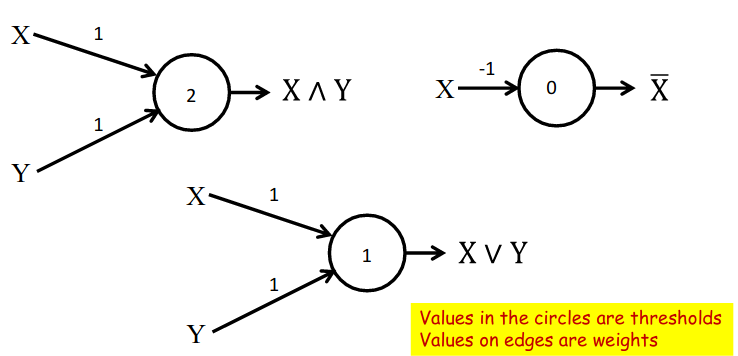
\includegraphics[width=0.7\linewidth, height=0.3\textheight]{img/gate}
	\caption{}
	\label{fig:gate}
\end{figure}


Figure 2 shows perceptron can compute AND, OR and NOT gates.Consider a perceptron for XOR gate with threshold $t$.
XOR gate is a digital logic gate that gives a true (1 or HIGH) output when the number of true inputs is odd. Let the  weights of  input be $w_1$ and $w_2$ and inputs be $X$ and $Y$. The input pairs  $(1,0)$, $(0,1)$, $(1,1)$, $(0,0)$ along with above threshold and weights have to hold  following inequalities for the perceptron to act as a XOR gate.

$$1w_1 + 0w_2 \geq t \implies w_1 \geq t$$
$$0w_1 + 1w_2 \geq t \implies w_2 \geq t$$
$$0w_1 + 0w_2 < t    \implies 0 < t$$
$$1w_1 + 1w_2 < t    \implies w_1 + w_2 <t $$

But these equations are in contradiction to each other. So a perceptron cannot compute an XOR gate.

A single perceptron(here, threshold gate) can be a Universal AND , OR and a majority gate.

\begin{figure}[h]
	\centering
	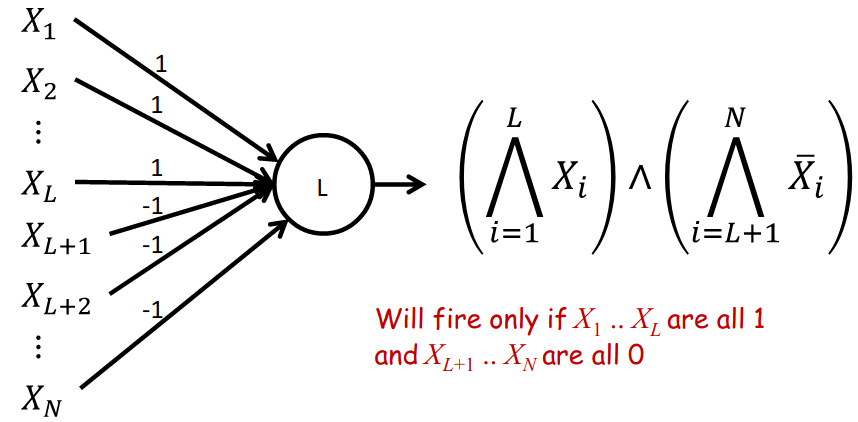
\includegraphics[width=0.4\linewidth]{img/and}
	\caption{Universal AND gate - AND any arbitrary number of inputs, of which any subset is negated}
	\label{fig:and}
\end{figure}

\begin{figure}[h]
	\centering
	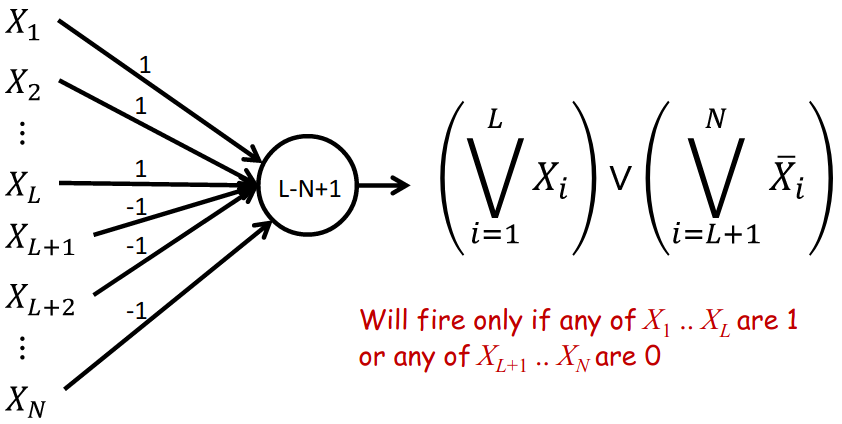
\includegraphics[width=0.4\linewidth]{img/or}
	\caption{Universal OR gate - OR any arbitrary number of inputs, of which any subset is negated}
	\label{fig:and}
\end{figure}

\begin{figure}[h]
	\centering
	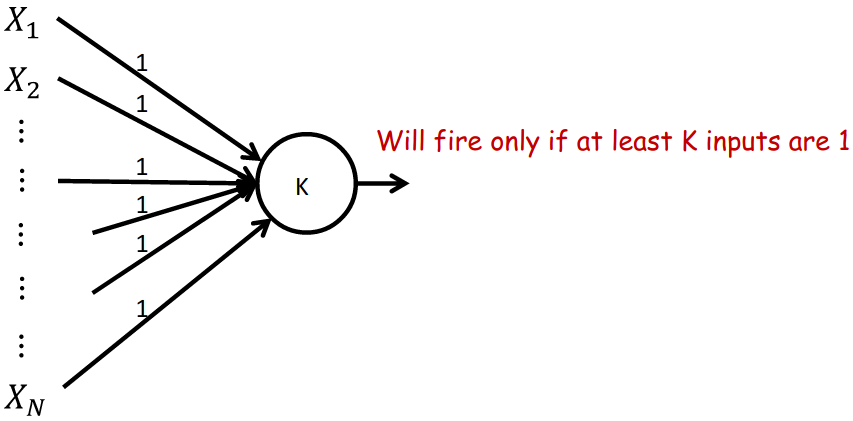
\includegraphics[width=0.4\linewidth]{img/majority}
	\caption{Generalized Majority gate - For implementing the same with standard boolean circuit would require exponentially (in input) sized cicuit, but can be done with single threshold gate }
	\label{fig:and}
\end{figure}

\cleardoublepage


\textbf{For any arbitrary Boolean function, how many layers of MLP is needed to compute it ?}
This  can be explained using Disjunctive Normal Forms(DNF) which is a canonical normal form of a logical formula consisting of  disjunction of conjunctions i.e OR of ANDs( sum of products)

Consider this Boolean function given as a truth table.This boolean function can be expressed as a DNF formula.This boolean function can be computed using a perceptron with a threshold activation.




	\begin{tabular}{|c|c|c|c|c|c|}
		\hline 
		$X_1$	& $X_2$ & $X_3$ &$X_4$  & $X_5$  & Y  \\ 
		\hline 
		0	& 0 & 1 & 1 & 0 & 1  \\ 
		\hline 
		0	&1  &  0& 1 &  1&1  \\ 
		\hline 
		0	& 1 &  1&  0&  0& 1 \\ 
		\hline 
		1	&  0&  0&  0&  1&  1\\ 
		\hline 
		1	&  0&  1&  1&  1& 1 \\ 
		\hline 
		1	& 1 &  0&  0&  1  & 1 \\
		\hline
		
		
	\end{tabular}
   
\begin{equation}
 \begin{split}
Y & = \overline{X_1} \  \overline{X_2}X_3X_4X_5  + \overline{X_1} X_2 \overline{X_3} X_4 X_5 \\
  & + \overline{X_1}X_2X_3\overline{X_4} \ \overline{X_5} +  X_1\overline{X_2} \ \overline{X_3} \ \overline{X_4} X_5 \\
  & + X_1 \overline{X_2} X_3X_4X_5 + X_1X_2 \overline{X_3} \ \overline{X_4} X_5    
  \end{split}
 \end{equation}





\begin{figure}[h]
	\centering
	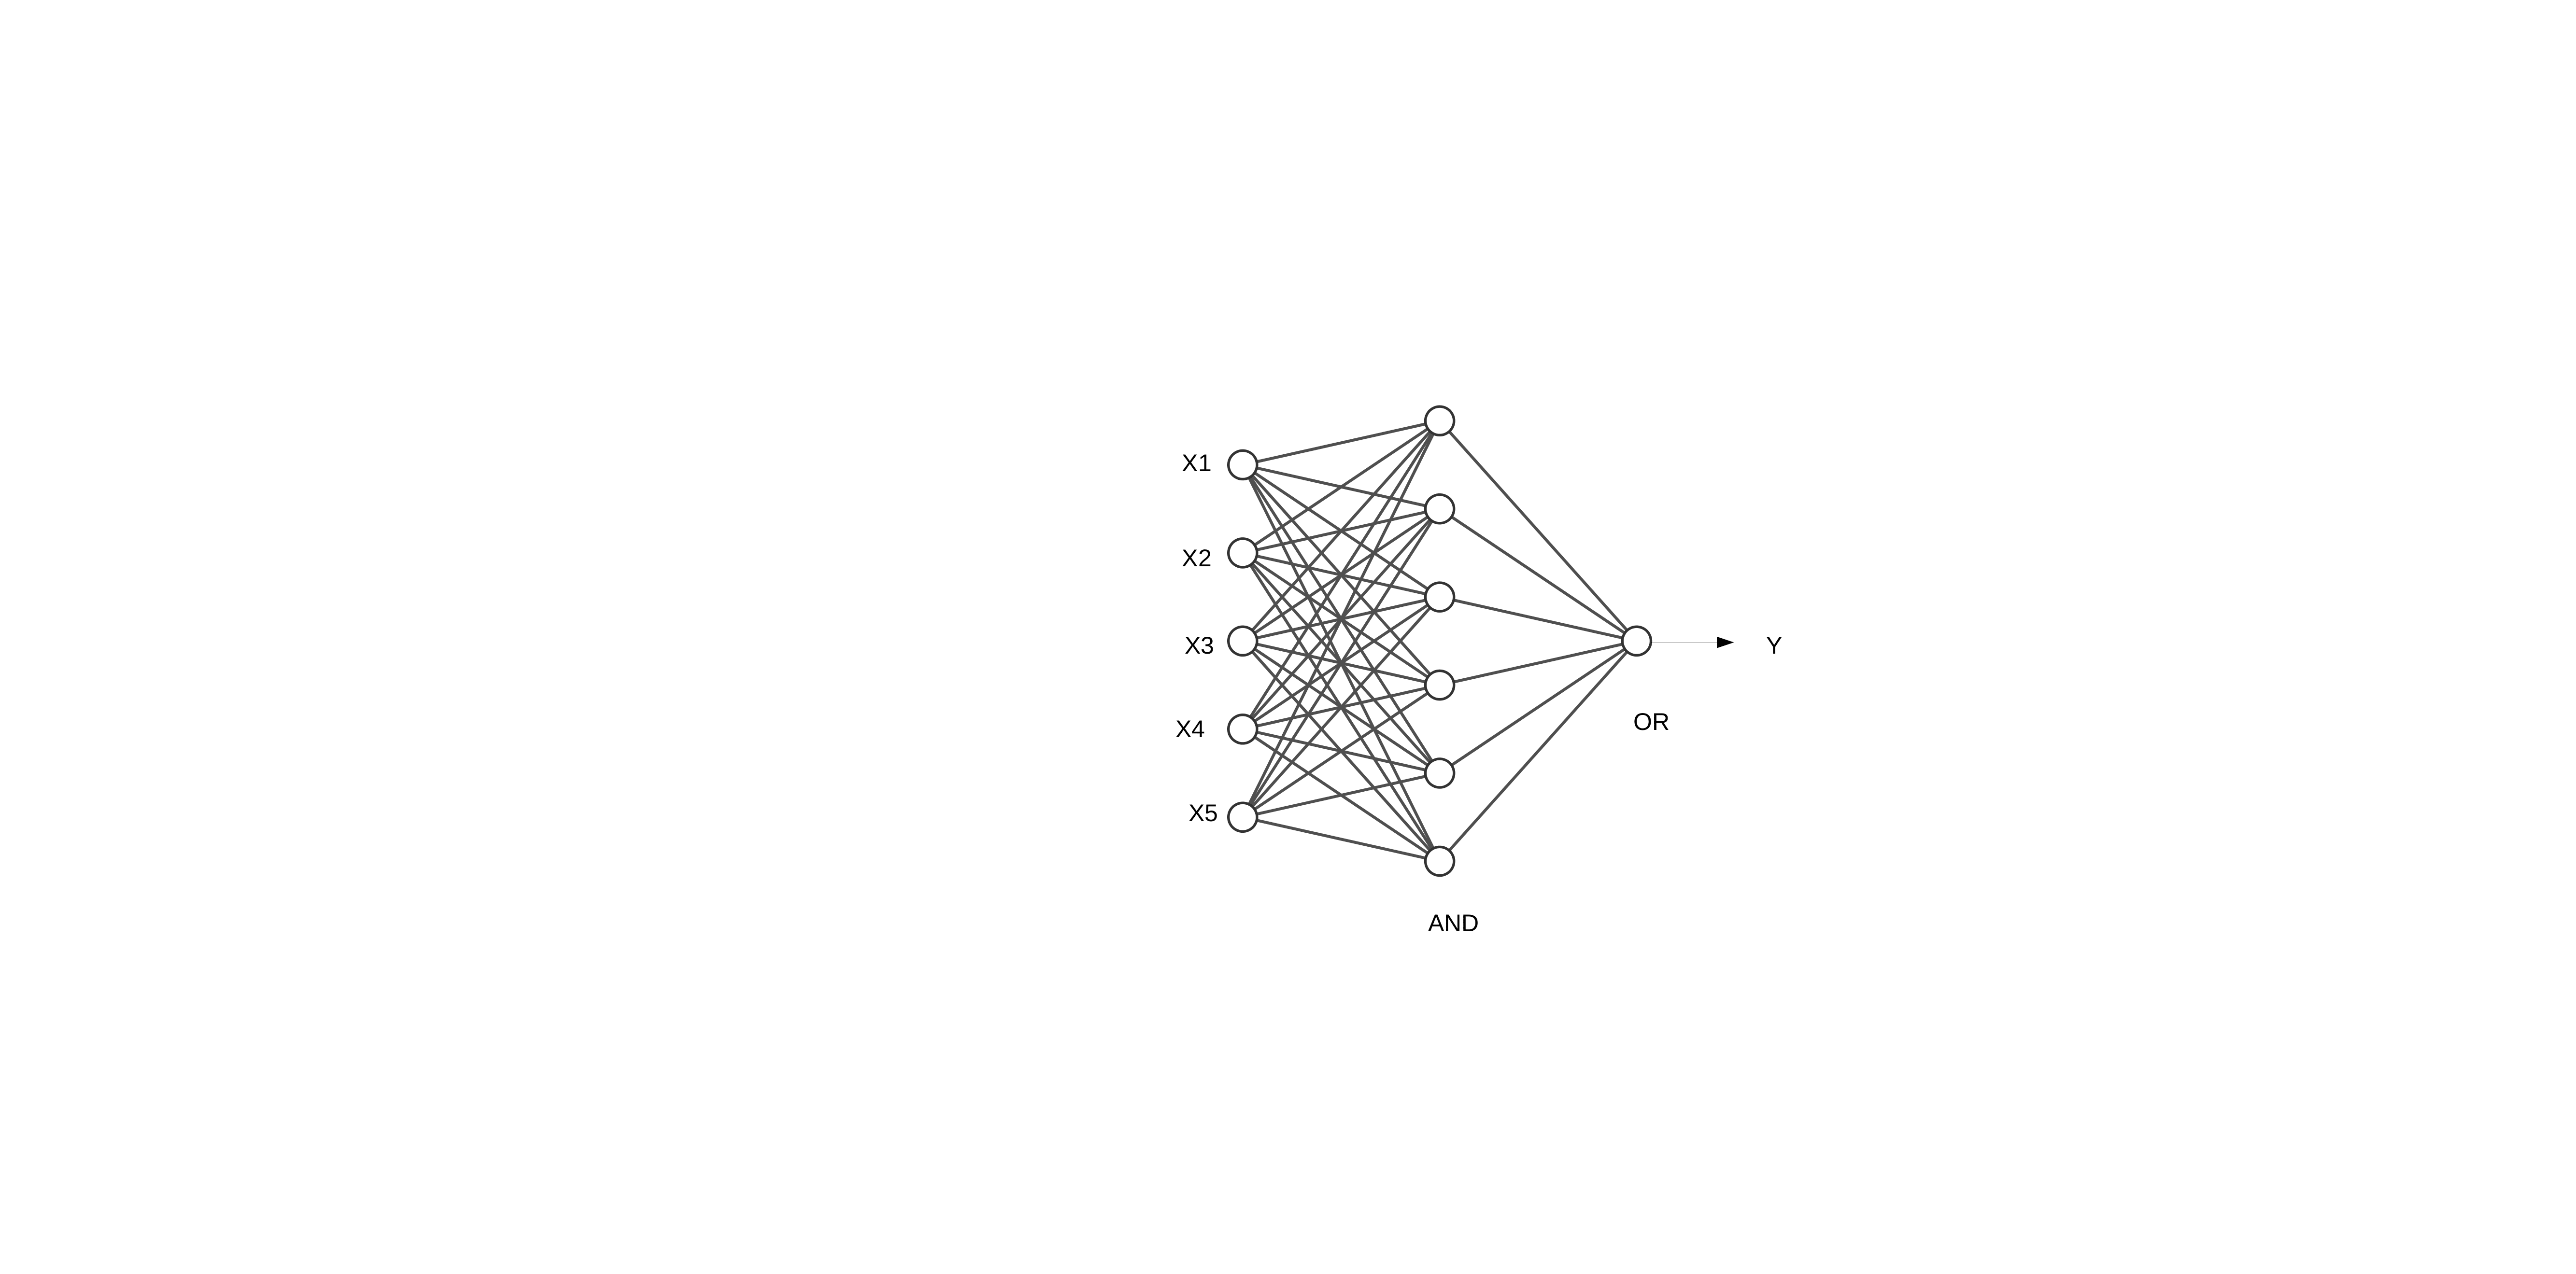
\includegraphics[width=1.1\linewidth]{img/nn-1}
\end{figure}







To be continued...

\cleardoublepage


\section{Learning}

Deep feedforward networks, also often called feedforward neural networks,
or multilayer perceptrons (MLPs), are the quintessential deep learning models.
The goal of a feedforward network is to approximate some function  $\textbf{g}$ . For example,
for a classifier, $ y = g (x)$ maps an input $x$ to a category $y$. A feedforward network
defines a mapping $y = f (x; W)$ and learns the value of the parameters W that result
in the best function approximation $f \approx g$.



So the neural network(NN) is a function approximator with parameters $W$, which must be set to appropriate values to get desired behaviour from the NN.For a given Neural Network (NN), the parameters are the weights and biases of the individual neuron. The learning process is finding the vales of the parameters such that the network computes the desired function.


\begin{figure}[ht]
	\centering
	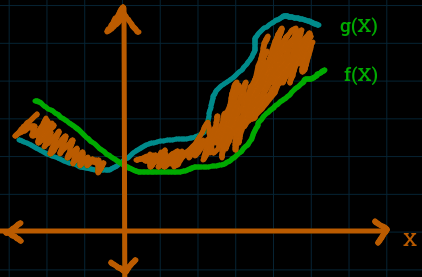
\includegraphics[width=0.5\linewidth]{img/error}
	\caption{Here, g(x) is the function we want the NN to  compute and f(x) is the funnction that we are computing}
	\label{fig:error}
\end{figure}

Error is the difference between $g(X)$ and $f(X)$ and the error waries with parameters. So the question of learnjng has reducredm to finding the parameters such that the error is less.When $f(x;W)$ has the capacity to exacly represent $g(x)$, we need to find $\hat{W}$, such that

$$ \hat{W} = argmin_W \int _x div(f(X;W), g(X)) dX$$
Where the $div(f(X;W), g(X)) = 0$ when $f(X;W) =  g(X)$. For finding the integral, $g(X)$ has to be fully specified inn the domain, but thats never the case.So we sample from the domain.

\begin{itemize}
	\item Get input-output pairs for a number of samples of $X_i$.
	\item Samples $(x_i, d_i)$ where $d_i = g(x_i) + noise $
	\item Optimum sampling when the samples of $X$ will be drawn using the distribution $P(X)$.
	\item eg: set of their images and their labels, speech recording and transcribes
\end{itemize}

Although $g(X)$ exists, we dont know the value of $g(X)$ throughout the domain of $g$, We only have value for the sampled points. What we do is, we learn the parameters of the NN such that it can fit the input-output pair we sampled i.e is the NN can correctly compute the $y$s for the $x$s we sampled and we hope the learned function $f(X;W)$ is same as the the original function $g(X)$ in the entire domain.


We  impose a  requirement - regions of the input space which has higher probability must have lower error than the regions of lower probabiltity.So we weigh the value of X with their probability distribution.

$$ \hat{W} = argmin_W \int _x div(f(X;W), g(X))P(X) dX$$
$$ \hat{W} = argmin_W \mathbb{E} \ [ div(f(X;W), g(X)) ]$$

The expected error(risk) is defined as the averaged error over the entire input space i.e,

$$\mathbb{E} \ [ div(f(X;W), g(X)) ] = \int _x div(f(X;W), g(X))P(X) dX $$
But its impossible to calculate the risk as $g(X)$ is unknown and what we have is just samples in the input space and their corresponding output. The emperical estimate of the expected error is the average error over all the samples, so, 

$$\mathbb{E} \ [ div(f(X;W), g(X)) ] = \frac{1}{N} \sum_{i = 1}^{N}  div(f(X_i;W), d_i = g(X_i))$$

This emperical average is known commonly as Loss,
$$L(W) = \frac{1}{N} \sum_{i = 1}^{N}  div(f(X_i;W), d_i = g(X_i))$$
So the problem now is to estimate the parameters to minimize the emperical estimate of expected error,

$$\hat{W} = argmin_W Loss(W)$$, So the problem now is an Optimization problem.


\end{document}